\section{Prediction by Partial Matching (PPM): The Statistical Pinnacle}

\begin{definitionbox}
Prediction by Partial Matching (PPM) is an adaptive statistical data compression
technique that uses a set of variable-length contexts to predict the next symbol
based on previously seen data. It dynamically builds models for contexts of
different lengths, favouring longer contexts when possible while falling back to
shorter ones to handle unseen patterns.
\end{definitionbox}

PPM was introduced by Cleary and Witten in 1984 and represents a breakthrough in
context-based modelling for lossless compression. By intelligently combining
multiple orders of Markov prediction, PPM achieves compression ratios close to the
theoretical entropy limits for many real-world data sources, such as text and binary
files.

\subsection{Introduction: Beyond Finite-Context Models}

\subsubsection{Recap of Markov Sources}

From Chapter~4.4, we recall that a Markov source of order $k$ models the probability
of the next symbol based solely on the previous $k$ symbols, known as the context $c$
with $|c| = k$. The conditional probability of symbol $s$ given $c$ is estimated as:
\[
    P(s \mid c)
    = \frac{\text{Count}(c, s)}{\displaystyle\sum_{s' \in \mathcal{A}} \text{Count}(c, s')},
\]
where $\mathcal{A}$ is the alphabet and $\text{Count}(c, s)$ is the number of times
symbol $s$ has followed context $c$ in the training data (or adaptively during
compression).

Fixed-order Markov models, while simple, suffer from significant limitations:
\begin{itemize}
    \item \textbf{Order-0 models:} Treat each symbol independently, ignoring all
          context. This yields near-uniform probabilities, leading to poor compression
          (e.g.\ 8~bits per symbol for ASCII text).
    \item \textbf{Low-order models} ($k = 1$ or $2$): Capture short-range dependencies
          (e.g.\ letter bigrams) but fail to exploit long-distance correlations, such as
          repeated phrases in natural language.
    \item \textbf{High-order models} ($k > 3$): Can model complex patterns but encounter
          the \textit{context sparsity problem}. With large alphabets
          (e.g.\ $|\mathcal{A}| = 256$ for byte data), most possible contexts never
          occur in finite data, resulting in zero-frequency estimates and unreliable
          predictions.
\end{itemize}

These issues motivate a more flexible approach that adapts the context length
dynamically.

\subsubsection{The Fundamental Insight}

The genius of PPM lies in its simple yet powerful principle: \textbf{attempt to use
the longest matching context available, but escape to shorter contexts if the current
one provides no information about the next symbol}.

\begin{importantbox}
PPM operates by maintaining a hierarchy of Markov models, from order-0 (no context)
up to a maximum order $M$ (typically $M = 3$ to $7$, depending on memory
constraints). To predict or encode a symbol, PPM begins with the highest-order
context (the last $M$ symbols). If that context has no record of the symbol (zero
frequency), it encodes an \textit{escape} event and descends to the next lower order
($M-1$), repeating until a matching context is found or order-0 is reached. This
ensures non-zero probabilities for all symbols.
\end{importantbox}

This multi-order strategy leverages:
\begin{itemize}
    \item \textbf{High-order contexts} for precise predictions in repetitive or
          structured data (e.g.\ \texttt{"the "} is often followed by common words).
    \item \textbf{Low-order fallbacks} for robustness against novel or sparse contexts.
    \item \textbf{Escape mechanism} to avoid zero probabilities, which would otherwise
          halt arithmetic coding.
\end{itemize}

The result is a predictor that approximates the true conditional entropy of the
source, often outperforming fixed-order models by 20--50\% on text data.

%=============================================================================
\subsection{The PPM Algorithm}
%=============================================================================

\subsubsection{Core Components}

PPM is typically paired with arithmetic coding (or range coding) for entropy
encoding, using the predicted probabilities to assign variable-length codes. The
model is \emph{adaptive}: probabilities update after each symbol is encoded or
decoded.

For each order $k = 0, 1, \ldots, M$, PPM maintains a context model storing:
\begin{itemize}
    \item A frequency table for symbols that have followed the context (only observed
          symbols are stored to save memory).
    \item Cumulative frequencies for efficient range selection in arithmetic coding.
    \item An \textit{escape weight} to estimate the probability of an unseen (novel)
          symbol.
\end{itemize}

Contexts are represented as strings consisting of the last $k$ symbols from the
history buffer.

\begin{definitionbox}
The \textbf{escape symbol} is a virtual event signalling that the next symbol is
unseen in the current context. Encoding or decoding the escape triggers a shift to
the lower-order model, where the process repeats. At order-0, escape indicates a
completely novel symbol in the entire stream, handled by a uniform distribution over
the unseen portion of the alphabet.
\end{definitionbox}

\begin{importantbox}
\textbf{Integration with Arithmetic Coding:}
The probabilities computed by PPM are fed directly into an arithmetic coder. 
For each coding step, the interval $[0,1)$ is partitioned according to the 
cumulative probabilities of all possible symbols (including escape) at the 
current context. The exclusion principle must be applied consistently in both 
the probability calculation and the interval partitioning.
\end{importantbox}

\subsubsection{The Escape and Prediction Mechanism}

The core challenge is estimating probabilities for unseen symbols without biasing
seen ones too heavily. PPM addresses the \textbf{zero-frequency problem} through
escape, but the escape probability itself must be carefully tuned.

Decoding is symmetric to encoding: the decoder uses the same context hierarchy and
probabilities to select the symbol, updating models identically.

\begin{algorithm}
\caption{PPM Prediction/Encoding Process (Simplified, for a Single Symbol)}
\begin{algorithmic}[1]
\Require Next symbol $x$ to encode, history buffer $H$, maximum order $M$,
         alphabet $\mathcal{A}$
\State $k \gets \min(M, |H|)$ \Comment{Available context length}
\State $seen \gets \emptyset$ \Comment{Track excluded symbols (exclusion principle)}
\While{$k \geq 0$}
    \State $c \gets$ last $k$ symbols of $H$
    \State Retrieve model for $c$: frequencies for $S_c$, total $N_c$, distinct $D_c$
    \State $S_{\mathrm{excl}} \gets S_c \cap seen$;\quad
           $N_{\mathrm{excl}} \gets \sum_{s \in S_{\mathrm{excl}}} \text{Count}(c,s)$
    \If{$x \in S_c \setminus S_{\mathrm{excl}}$}
        \State $P(x \mid c, \mathit{excl}) \gets
               \dfrac{\text{Count}(c,x)}{N_c + E_c}$
               \Comment{$E_c$ is the escape weight}
        \State Encode $x$ using this probability
        \State $\text{Count}(c,x) \gets \text{Count}(c,x) + 1$
        \State \textbf{return}
    \Else
        \State $P(\text{escape} \mid c, \mathit{excl}) \gets
               \dfrac{E_c}{N_c + E_c}$
        \State Encode escape using this probability
        \State $seen \gets seen \cup (S_c \setminus S_{\mathrm{excl}})$
        \State $k \gets k - 1$
    \EndIf
\EndWhile
\If{$k < 0$}
    \State $U \gets |\mathcal{A}| - |seen|$ \Comment{Number of truly unseen symbols}
    \State $P(x \mid \mathit{unseen}) \gets 1/U$
    \State Encode $x$ using this uniform probability
    \State Update order-0 model with $x$
\EndIf
\State Append $x$ to $H$; truncate $H$ to the last $M$ symbols
\end{algorithmic}
\end{algorithm}

\subsubsection{Escape Estimation Methods}

The escape weight $E_c$ is critical to performance. Early PPM variants used simple
heuristics; later ones refined them considerably.

%-----------------------------------------------------------------------------
\paragraph{Method~A (PPMA): Fixed Escape}

\begin{definitionbox}
\textbf{Method~A} assumes a single unseen symbol at all times, setting $E_c = 1$
regardless of $D_c$:
\[
    P(\text{escape} \mid c) = \frac{1}{N_c + 1},
    \qquad
    P(s \mid c) = \frac{\text{Count}(c,s)}{N_c + 1}
    \quad \forall\, s \in S_c.
\]
\end{definitionbox}

This is computationally trivial but statistically naive: it overestimates escape
probability when many symbols have been seen ($D_c \approx |\mathcal{A}|$) and
underestimates it when the context is still being populated.

%-----------------------------------------------------------------------------
\paragraph{Method~B (PPMB): Proportional to Distinct Symbols}

\begin{definitionbox}
\textbf{Method~B} sets $E_c = D_c$, reflecting the intuition that the likelihood of
seeing a novel symbol grows with the diversity already observed:
\[
    P(\text{escape} \mid c) = \frac{D_c}{N_c + D_c},
    \qquad
    P(s \mid c) = \frac{\text{Count}(c,s)}{N_c + D_c}.
\]
\end{definitionbox}

Method~B is more adaptive than Method~A but can still underestimate escape in sparse
contexts, where small counts give a misleadingly confident distribution.

%-----------------------------------------------------------------------------
\paragraph{Method~C (PPMC): Standard Heuristic}

\begin{definitionbox}
\textbf{Method~C} (the most widely used variant) sets $E_c = D_c$, the same as Method~B, 
but with explicit handling of edge cases and a different philosophical justification. 
For an empty context ($D_c = 0$), the entire probability mass is placed on the escape event. 
The formulas are identical to Method~B:
\[
    P(\text{escape} \mid c) = \frac{D_c}{N_c + D_c},
    \qquad
    P(s \mid c) = \frac{\text{Count}(c,s)}{N_c + D_c}.
\]

The key difference is that PPMC treats the escape probability as representing the 
probability of a \emph{novel} symbol, while Method~B's justification was based on 
counting distinct symbols. In practice, PPMC became the standard because it performs 
well across diverse data types.
\end{definitionbox}

One can verify that probabilities always sum to~1:
\[
    \sum_{s \in S_c} \frac{\text{Count}(c,s)}{N_c + D_c}
    + \frac{D_c}{N_c + D_c}
    = \frac{N_c + D_c}{N_c + D_c} = 1.
\]

%-----------------------------------------------------------------------------
\paragraph{Method~D (PPMD): Advanced Estimation}

\begin{definitionbox}
\textbf{Method~D} uses a dynamically computed escape weight informed by
\emph{singleton} symbols --- those with count equal to~1. A common formulation is:
\[
    E_c = \max\left(1,\; \frac{\#\{s : \text{Count}(c,s)=1\}}{N_c} \cdot |\mathcal{A}|\right)
\]
or more simply:
\[
    E_c = \frac{\#\{s : \text{Count}(c,s)=1\}}{N_c} \cdot D_c
\]
with a lower bound of 1 to ensure $P(\text{escape}) > 0$.

Full PPMD implementations employ \emph{Secondary Escape Estimation} (SEE), which
uses a separate statistical model to predict $P(\text{escape})$ from context
features such as $D_c$, $N_c$, and order.
\end{definitionbox}

PPMD reduces bias in non-stationary data at the cost of increased implementation
complexity.

\begin{examplebox}
\textbf{Numeric comparison of methods.}
Suppose a context has $N_c = 5$ total observations and $D_c = 3$ distinct symbols
with counts $[3, 1, 1]$.
\begin{center}
\begin{tabular}{lcccc}
\toprule
Method & $E_c$ & Denominator & $P(\text{escape})$ & $P(s_1)$ \\
\midrule
A & $1$ & $6$  & $1/6  \approx 0.167$ & $3/6 = 0.500$ \\
B & $3$ & $8$  & $3/8  = 0.375$       & $3/8 = 0.375$ \\
C & $3$ & $8$  & $3/8  = 0.375$       & $3/8 = 0.375$ \\
D & $2$ & $7$  & $2/7  \approx 0.286$ & $3/7 \approx 0.429$ \\
\bottomrule
\end{tabular}
\end{center}
For Method~D, with 2 singletons out of 5 observations, a simple formula gives
$E_c = (2/5) \times 3 = 1.2 \approx 2$ (rounded up to integer for simplicity).
Method~A over-trusts the context; Methods~B and~C give a substantial escape
allocation; Method~D lies in between based on singleton proportion.
\end{examplebox}

\subsubsection{The Exclusion Principle}

\begin{importantbox}
The \textbf{exclusion principle} is a key optimisation in PPM: when the encoder
escapes from a higher-order context to a lower-order one, all symbols that were
\emph{present} in the higher-order context (and hence already considered) are
\emph{excluded} from the probability distribution in the lower-order context. This
renormalises the remaining probabilities upward, sharpening predictions for
genuinely novel symbols and typically saving 5--10\% of bits compared with
non-excluding PPM.
\end{importantbox}

\begin{examplebox}
\textbf{Quantified exclusion.}
Suppose order-2 context \texttt{"ab"} has seen $\{$\texttt{r}$\}$ only, so an escape
is sent. The order-1 context \texttt{"b"} has seen $\{$\texttt{r}, \texttt{a}$\}$
with counts $[1,1]$ ($N=2$, $D=2$).
\begin{itemize}
    \item \emph{Without exclusion:} $P(\texttt{r}) = 1/4$,
          $P(\texttt{a}) = 1/4$, $P(\text{esc}) = 2/4 = 0.5$.
    \item \emph{With exclusion} of \texttt{r} ($S_{\mathrm{excl}} = \{\texttt{r}\}$,
          remaining $D_{\mathrm{eff}}=1$, $N_{\mathrm{eff}}=1$):
          $P(\texttt{a}) = 1/2$, $P(\text{esc}) = 1/2$.
\end{itemize}
Excluding \texttt{r} doubles $P(\texttt{a})$, saving $1$ bit if \texttt{a} is the
next symbol.
\end{examplebox}

%=============================================================================
\subsection{Step-by-Step Examples}
%=============================================================================

We trace the encoding of two strings using PPMC with $M = 2$ and alphabet size
$|\mathcal{A}| = 256$ (bytes). Arithmetic coding is assumed; ideal code length
$\approx -\log_2 P$ bits. Models update after each symbol. For novel symbols at
order-($-1$), we approximate the fallback uniform probability as $1/256$ for
bit-length calculations (the true denominator is $|\mathcal{A}| - |seen|$, which
causes only a small error early in the stream).

%-----------------------------------------------------------------------------
\subsubsection{Example 1: Encoding \texttt{"abracadabra"} (No Exclusion)}

\paragraph{Initialisation.} All models empty. History $H = \varepsilon$.

\bigskip
\noindent\textbf{Symbol 1: \texttt{'a'}}\\
No context available; use uniform. $P(\texttt{a}) = 1/256 \approx 8$ bits.\\
Update: Order-0: \texttt{a}:1, $D_0=1$, $N_0=1$. $H =$ \texttt{a}.

\bigskip
\noindent\textbf{Symbol 2: \texttt{'b'}}\\
$k_{\max}=1$.
\begin{itemize}
    \item Order-1 \texttt{(a)}: empty $\Rightarrow$ escape (0 bits, probability = 1).
    \item Order-0: $D_0=1$, $N_0=1$; $P(\text{esc})=1/2$ (1 bit).
          \texttt{b} unseen $\Rightarrow$ escape.
    \item Fallback: $P(\texttt{b}) \approx 1/256 \approx 8$ bits.
\end{itemize}
\textbf{Total} $\approx 1 + 8 = 9$ bits.\\
Update: O-1(\texttt{a}): \texttt{b}:1; O-0: \texttt{b}:1 ($D_0=2$, $N_0=2$).
$H =$ \texttt{ab}.

\bigskip
\noindent\textbf{Symbol 3: \texttt{'r'}}\\
$k_{\max}=2$.
\begin{itemize}
    \item Order-2 \texttt{(ab)}: empty $\Rightarrow$ escape (0 bits).
    \item Order-1 \texttt{(b)}: empty $\Rightarrow$ escape (0 bits).
    \item Order-0: $D_0=2$, $N_0=2$; $P(\text{esc})=2/4=0.5$ (1 bit).
          \texttt{r} unseen $\Rightarrow$ escape.
    \item Fallback: $\approx 8$ bits.
\end{itemize}
\textbf{Total} $\approx 1 + 8 = 9$ bits.\\
Update: O-2(\texttt{ab}):\texttt{r}:1; O-1(\texttt{b}):\texttt{r}:1;
O-0: \texttt{r}:1 ($D_0=3$, $N_0=3$). $H =$ \texttt{abr}.

\bigskip
\noindent\textbf{Symbol 4: \texttt{'a'}}\\
$H =$ \texttt{abr}.
\begin{itemize}
    \item Order-2 \texttt{(br)}: empty $\Rightarrow$ escape (0 bits).
    \item Order-1 \texttt{(r)}: empty $\Rightarrow$ escape (0 bits).
    \item Order-0: \texttt{a}:1, $D_0=3$, $N_0=3$; denom $= 3+3=6$.
          $P(\texttt{a}) = 1/6 \approx 2.58$ bits. \texttt{a} found.
\end{itemize}
\textbf{Total} $\approx 2.58$ bits.\\
Update: O-2(\texttt{br}):\texttt{a}:1; O-1(\texttt{r}):\texttt{a}:1;
O-0: \texttt{a}:2 ($N_0=4$). $H =$ \texttt{abra}.

\bigskip
\noindent\textbf{Symbol 5: \texttt{'c'}}\\
$H =$ \texttt{abra}.
\begin{itemize}
    \item Order-2 \texttt{(ra)}: empty $\Rightarrow$ escape (0 bits).
    \item Order-1 \texttt{(a)}: \texttt{b}:1 ($D=1$, $N=1$); denom $=2$.
          $P(\text{esc})=1/2 \approx 1$ bit. \texttt{c} unseen.
    \item Order-0: $D_0=3$, $N_0=4$; denom $=7$.
          $P(\text{esc})=3/7 \approx 1.22$ bits. \texttt{c} unseen.
    \item Fallback: $\approx 8$ bits.
\end{itemize}
\textbf{Total} $\approx 1 + 1.22 + 8 = 10.22$ bits.\\
Update: \texttt{c} added to all models; $D_0=4$, $N_0=5$. $H =$ \texttt{abrac}.

\bigskip
\noindent\textbf{Symbol 6: \texttt{'a'}}\\
$H =$ \texttt{abrac}.
\begin{itemize}
    \item Order-2 \texttt{(ac)}: empty $\Rightarrow$ escape (0 bits).
    \item Order-1 \texttt{(c)}: empty $\Rightarrow$ escape (0 bits).
    \item Order-0: \texttt{a}:2, $D_0=4$, $N_0=5$; denom $=9$.
          $P(\texttt{a})=2/9 \approx 2.17$ bits.
\end{itemize}
\textbf{Total} $\approx 2.17$ bits.\\
Update: O-0: \texttt{a}:3 ($N_0=6$). $H =$ \texttt{abraca}.

\bigskip
\noindent\textbf{Symbol 7: \texttt{'d'}}\\
$H =$ \texttt{abraca}.
\begin{itemize}
    \item Order-2 \texttt{(ca)}: empty $\Rightarrow$ escape (0 bits).
    \item Order-1 \texttt{(a)}: \texttt{b}:1, \texttt{c}:1 ($D=2$, $N=2$);
          denom $=4$. $P(\text{esc})=2/4=0.5 \approx 1$ bit. \texttt{d} unseen.
    \item Order-0: $D_0=4$, $N_0=6$; denom $=10$.
          $P(\text{esc})=4/10=0.4 \approx 1.32$ bits. \texttt{d} unseen.
    \item Fallback: $\approx 8$ bits.
\end{itemize}
\textbf{Total} $\approx 1 + 1.32 + 8 = 10.32$ bits.\\
Update: \texttt{d} added; $D_0=5$, $N_0=7$. $H =$ \texttt{abracad}.

\bigskip
\noindent\textbf{Symbol 8: \texttt{'a'}}\\
$H =$ \texttt{abracad}.
\begin{itemize}
    \item Order-2 \texttt{(ad)}: empty $\Rightarrow$ escape (0 bits).
    \item Order-1 \texttt{(d)}: empty $\Rightarrow$ escape (0 bits).
    \item Order-0: \texttt{a}:3, $D_0=5$, $N_0=7$; denom $=12$.
          $P(\texttt{a})=3/12=0.25 \approx 2$ bits.
\end{itemize}
\textbf{Total} $\approx 2$ bits.\\
Update: O-0: \texttt{a}:4 ($N_0=8$). $H =$ \texttt{abracada}.

\bigskip
\noindent\textbf{Symbol 9: \texttt{'b'}}\\
$H =$ \texttt{abracada}.
\begin{itemize}
    \item Order-2 \texttt{(da)}: empty $\Rightarrow$ escape (0 bits).
    \item Order-1 \texttt{(a)}: \texttt{b}:1, \texttt{c}:1, \texttt{d}:1
          ($D=3$, $N=3$); denom $=6$.
          $P(\texttt{b})=1/6 \approx 2.58$ bits. \texttt{b} found.
\end{itemize}
\textbf{Total} $\approx 2.58$ bits.\\
Update: O-1(\texttt{a}): \texttt{b}:2 ($N=4$); O-0: \texttt{b}:2 ($N_0=9$).
$H =$ \texttt{abracadab}.

\bigskip
\noindent\textbf{Symbol 10: \texttt{'r'}}\\
$H =$ \texttt{abracadab}.
\begin{itemize}
    \item Order-2 \texttt{(ab)}: \texttt{r}:1 ($D=1$, $N=1$); denom $=2$.
          $P(\texttt{r})=1/2 = 1$ bit. \texttt{r} found.
\end{itemize}
\textbf{Total} $= 1$ bit.\\
Update: O-2(\texttt{ab}): \texttt{r}:2; O-0: \texttt{r}:2 ($N_0=10$).
$H =$ \texttt{abracadabr}.

\bigskip
\noindent\textbf{Symbol 11: \texttt{'a'}}\\
$H =$ \texttt{abracadabr}.
\begin{itemize}
    \item Order-2 \texttt{(br)}: \texttt{a}:1 ($D=1$, $N=1$); denom $=2$.
          $P(\texttt{a})=1/2 = 1$ bit.
\end{itemize}
\textbf{Total} $= 1$ bit.\\
Update: O-2(\texttt{br}): \texttt{a}:2; O-0: \texttt{a}:5.

\bigskip
\noindent\textbf{Summary (Example~1).}
\begin{verbatim}
Symbol | Code bits (approx)
-------+--------------------
  a    |  8.00  (uniform fallback)
  b    |  9.00  (2 escapes + uniform)
  r    |  9.00  (3 escapes + uniform)
  a    |  2.58  (2 escapes + order-0)
  c    | 10.22  (3 escapes + uniform)
  a    |  2.17  (2 escapes + order-0)
  d    | 10.32  (3 escapes + uniform)
  a    |  2.00  (2 escapes + order-0)
  b    |  2.58  (1 escape  + order-1)
  r    |  1.00  (order-2 hit)
  a    |  1.00  (order-2 hit)
-------+--------------------
Total  | ~57.87 bits  vs  88 bits raw ASCII
\end{verbatim}

The final two symbols, encoded with only $1$ bit each, demonstrate the power of PPM:
once a two-gram has been seen, re-encoding it becomes highly efficient.

%-----------------------------------------------------------------------------
\subsubsection{Example 2: Repetitive String \texttt{"ababababab"} ($M=1$, PPMC)}

This example shows how order-1 PPM rapidly learns a strict alternation pattern.
Alphabet size 256; $M=1$ (order-0 and order-1 only).

\bigskip
\noindent\textbf{Symbol 1 -- \texttt{'a'}:} uniform, $\approx 8$ bits.
O-0: \texttt{a}:1. $H=$ \texttt{a}.

\noindent\textbf{Symbol 2 -- \texttt{'b'}:} O-1(\texttt{a}) empty, esc; O-0
$P(\text{esc})=1/2$ (1~bit), \texttt{b} unseen $\Rightarrow$ fallback 8~bits.
Total $\approx 9$ bits.
O-1(\texttt{a}):\texttt{b}:1; O-0:\texttt{b}:1.

\noindent\textbf{Symbol 3 -- \texttt{'a'}:} O-1(\texttt{b}) empty, esc;
O-0: \texttt{a}:1 of 2, denom 4, $P(\texttt{a})=1/4 = 2$ bits.

\noindent\textbf{Symbol 4 -- \texttt{'b'}:} O-1(\texttt{a}):\texttt{b}:1
($D=1$, $N=1$), $P(\texttt{b})=1/2 = 1$ bit.

\noindent\textbf{Symbol 5 -- \texttt{'a'}:} O-1(\texttt{b}):\texttt{a}:1
(updated after sym~3), $P(\texttt{a})=1/2 = 1$ bit.

\noindent\textbf{Symbol 6 -- \texttt{'b'}:} O-1(\texttt{a}):\texttt{b}:2
($D=1$, $N=2$), $P(\texttt{b})=2/3 \approx 0.58$ bits.

\noindent\textbf{Symbol 7 -- \texttt{'a'}:} O-1(\texttt{b}):\texttt{a}:2,
$P(\texttt{a})=2/3 \approx 0.58$ bits.

\noindent\textbf{Symbol 8 -- \texttt{'b'}:} O-1(\texttt{a}):\texttt{b}:3,
$P(\texttt{b})=3/4 \approx 0.42$ bits.

\noindent\textbf{Symbol 9 -- \texttt{'a'}:} O-1(\texttt{b}):\texttt{a}:3,
$P(\texttt{a})=3/4 \approx 0.42$ bits.

\noindent\textbf{Symbol 10 -- \texttt{'b'}:} O-1(\texttt{a}):\texttt{b}:4,
$P(\texttt{b})=4/5 \approx 0.32$ bits.

\bigskip
\textbf{Total} $\approx 8+9+2+1+1+0.58+0.58+0.42+0.42+0.32 \approx 23.3$ bits
($2.33$ bpc).\\
An adaptive order-0 model gives $\approx 1$ bpc once stabilised but requires far
more symbols; PPM-1 reaches near-optimal coding by symbol~5 due to the strict
alternation captured by the order-1 context.

%-----------------------------------------------------------------------------
\subsubsection{Example 3: Exclusion Applied to \texttt{"abracadabra"} (Symbol~5)}

We revisit symbol~5 (\texttt{'c'}) from Example~1 but now apply exclusion.

After encoding symbols 1--4 (\texttt{"abra"}), the relevant models are:
\begin{itemize}
    \item Order-2 \texttt{(ra)}: empty.
    \item Order-1 \texttt{(a)}: \texttt{b}:1 ($D=1$, $N=1$).
    \item Order-0: \texttt{a}:2, \texttt{b}:1, \texttt{r}:1 ($D=3$, $N=4$).
\end{itemize}

\textbf{Step 1 --- Order-2 escape.} \texttt{(ra)} is empty, $P(\text{esc})=1$.
Symbols excluded from lower orders: $\emptyset$.

\textbf{Step 2 --- Order-1 escape with exclusion.} \texttt{(a)} contains
\texttt{b}:1 only. \texttt{c} is not present $\Rightarrow$ escape.
$P(\text{esc}) = 1/2$ (1~bit). After this step, $seen = \{\texttt{b}\}$.

\textbf{Step 3 --- Order-0 with exclusion of \texttt{b}.} Effective table:
\texttt{a}:2, \texttt{r}:1 (exclude \texttt{b}). $D_{\mathrm{eff}}=2$,
$N_{\mathrm{eff}}=3$; denom $= 3+2 = 5$.
$P(\text{esc}) = 2/5$ ($\approx 1.32$ bits). \texttt{c} unseen $\Rightarrow$ escape.

\textbf{Without exclusion} (Example~1): $P(\text{esc at O-0}) = 3/7 \approx 1.22$
bits.\\
\textbf{With exclusion}: $P(\text{esc at O-0}) = 2/5 = 1.32$ bits.

Here exclusion slightly increases the O-0 escape cost, but crucially, if the target
symbol had been \texttt{a}, exclusion would have increased $P(\texttt{a})$ from
$2/7 \approx 1.81$ bits to $2/5 = 1.32$ bits --- a saving of $0.49$ bits. Exclusion
benefits the \emph{average} case by concentrating probability on likely symbols.

%=============================================================================
\subsection{PPM Implementation Challenges}
%=============================================================================

\subsubsection{Memory Management}

High-order PPM can, in the worst case, require up to $|\mathcal{A}|^M$ contexts.

\begin{examplebox}
For $M = 5$ and $|\mathcal{A}| = 256$ (byte data), the theoretical maximum is
$256^5 \approx 1.1 \times 10^{12}$ contexts --- clearly infeasible. However, on
typical English text ($|\mathcal{A}| \approx 70$ printable characters), the actual
number of observed contexts stays below $10^6$ with 1~MB of RAM. PPM exploits this
sparsity by allocating memory only for contexts actually encountered.
\end{examplebox}

Memory is managed through:
\begin{itemize}
    \item \textbf{Lazy allocation}: Context nodes are created on first encounter.
    \item \textbf{Count rescaling}: Periodically halving all counts prevents overflow
          and lets the model adapt to non-stationary data.
    \item \textbf{Memory budgets}: Some implementations cap total nodes and evict the
          least-recently-used contexts when full.
\end{itemize}

\subsubsection{Data Structures: The Context Trie}

The standard solution for efficient context lookup is a \textbf{trie} (prefix tree).

\begin{definitionbox}
In a \textbf{context trie}, the root node represents the empty context (order-0).
Each edge is labelled with a symbol, and a path of length $k$ from the root
represents a $k$-th order context. Each node stores:
\begin{itemize}
    \item A (sparse) frequency array for symbols following this context.
    \item An escape weight.
    \item Child pointers (typically a hash map for large alphabets).
    \item A \emph{suffix link} pointing to the node for the context obtained by
          dropping the oldest symbol, enabling O(1) fallback.
\end{itemize}
\end{definitionbox}

Suffix links allow PPM to traverse the escape hierarchy in $O(M)$ time without
rebuilding the context string at each level. Combined with hashed children, the trie
supports $O(1)$ average-case lookup and update.

\begin{figure}[h]
\centering
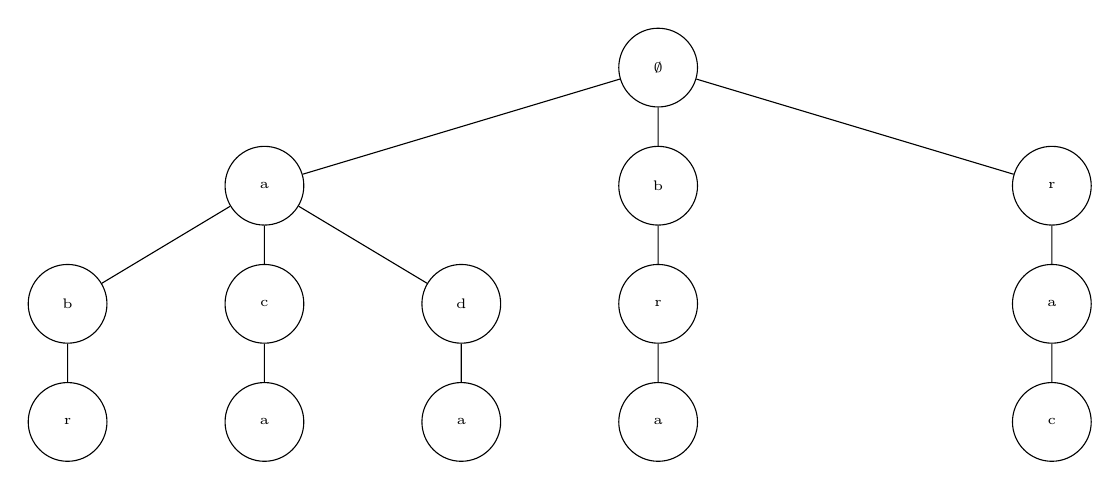
\begin{tikzpicture}[
    level distance=1.5cm,
    level 1/.style={sibling distance=5cm},
    level 2/.style={sibling distance=2.5cm},
    every node/.style={circle, draw, minimum size=1cm, font=\tiny}
]
\node (root) {$\emptyset$}
    child {node {a}
        child {node {b}
            child {node {r}}
        }
        child {node {c}
            child {node {a}}
        }
        child {node {d}
            child {node {a}}
        }
    }
    child {node {b}
        child {node {r}
            child {node {a}}
        }
    }
    child {node {r}
        child {node {a}
            child {node {c}}
        }
    };
\end{tikzpicture}
\caption{Partial context trie for \texttt{"abracadabra"} with $M=3$. Each path from
the root to a node at depth $k$ represents a $k$-th order context; suffix links
(not shown) connect each depth-$k$ node to the depth-$(k-1)$ node for the same
context suffix. This structure enables $O(1)$ escape transitions.}
\label{fig:context-trie}
\end{figure}

\subsubsection{The Zero-Frequency Problem and Modern Refinements}

Several advanced techniques address the remaining inadequacies of simple escape
estimation:
\begin{itemize}
    \item \textbf{Adaptive escape}: Adjust escape weight online using running averages
          of how often escape was actually needed in each context class.
    \item \textbf{Secondary Escape Estimation (SEE)}: Use a second-level model (often
          itself a PPM-like structure over context metadata) to predict
          $P(\text{escape})$; used in PPMZ and PAQ.
    \item \textbf{Universal coding connections}: View escape as coding the event
          ``novel symbol''; Bayesian methods (e.g.\ Krichevsky--Trofimov estimator)
          give principled priors.
    \item \textbf{Mixing}: Combine escape estimates from different orders via
          log-linear interpolation (foreshadowing context mixing, Section~5.3).
\end{itemize}

%=============================================================================
\subsection{PPM Variants and Successors}
%=============================================================================

\subsubsection{PPM*: Unbounded Contexts}

\begin{definitionbox}
\textbf{PPM*} (Witten, Neal, and Cleary, 1987) removes the fixed maximum order $M$,
instead finding the longest suffix of the current history that has been seen at least
once in the past. This is analogous to the phrase-matching in Ziv--Lempel (LZ)
schemes but operates probabilistically.
\end{definitionbox}

PPM* is implemented efficiently using augmented tries with \emph{failure functions}
(similar to Aho--Corasick), achieving $O(n \log n)$ compression time.

\begin{examplebox}
On the string \texttt{"banana"}, suppose the full context \texttt{"anana"} was
seen during encoding. PPM* would use this five-symbol context, whereas PPM with
$M=3$ would be limited to \texttt{"ana"} --- potentially missing stronger
long-range predictions.
\end{examplebox}

\textbf{Trade-off:} PPM* excels on long-period repetitive data (DNA, source code)
but may over-fit on noisy or short data, where shorter fixed contexts provide more
reliable statistics (see Exercise~4.3).

\subsubsection{PPMZ: Optimised Practical Variant}

Building on PPMC, Charles Bloom's PPMZ introduced several production-quality
innovations:
\begin{itemize}
    \item \textbf{Dynamic order selection}: The effective maximum order adapts
          per-block based on measured prediction improvement.
    \item \textbf{Secondary Escape Estimation (SEE)}: A compact neural-like model
          replaces fixed heuristics for $P(\text{escape})$, updating on-the-fly.
    \item \textbf{Weighted novelty}: Unseen symbols at the fallback level are
          assigned probabilities biased toward frequently appearing symbols in the
          global distribution.
\end{itemize}

PPMZ held world records on the Calgary Corpus throughout the late 1990s, outperforming
Gzip and BZIP2 by 20--30\%.

\subsubsection{PAQ: Context Mixing}

\begin{importantbox}
\textbf{Context mixing} represents the natural evolution of PPM's multi-order
philosophy. Rather than \emph{escaping} through a hierarchy, PAQ (Matt Mahoney,
2002) \emph{combines} predictions from all orders simultaneously using adaptive
weighting.
\end{importantbox}

Key innovations in PAQ and its descendants:
\begin{itemize}
    \item \textbf{Hundreds of models}: Order-0 through order-12 PPM models, plus
          word-level models, sparse contexts, and transform-based models
          (e.g.\ BWT residuals).
    \item \textbf{Log-linear mixing}: Each model outputs a log-odds prediction
          $\ell_i = \log \frac{P_i(1)}{P_i(0)}$; the combined prediction is
          \[
              P_{\text{mix}}(1) = \sigma\!\left(\sum_i w_i \ell_i\right),
              \quad \sigma(x) = \frac{1}{1+e^{-x}}.
          \]
    \item \textbf{Online weight update}: Weights $w_i$ increase for models that
          predicted the actual symbol and decrease otherwise (gradient descent on
          log-loss).
\end{itemize}

PAQ8 and its successor CMIX consistently win the Hutter Prize (enwik9, 100~MB
Wikipedia), achieving $\approx 1.1$--$1.3$ bpc on English, within 10--30\% of the
estimated Shannon limit of $\approx 1.0$ bpc.

\begin{examplebox}
In PAQ encoding a space after \texttt{"the"}: the order-3 model assigns
$P(\text{space}) = 0.40$, a word-boundary model assigns $0.65$, a positional model
$0.35$. Mixed log-linearly with learned weights, the combined
$P(\text{space}) \approx 0.55$ --- better than any single model alone.
\end{examplebox}

\subsubsection{Limitations of PPM}

Despite its theoretical elegance, PPM has practical limitations:

\begin{itemize}
    \item \textbf{Memory consumption}: Even with trie structures, PPM with $M=5$ can 
          consume hundreds of megabytes on large files, limiting its use in memory-constrained 
          environments.
    \item \textbf{Speed}: Context lookups and updates are slower than dictionary-based 
          methods like LZ77, making PPM impractical for real-time or high-throughput applications.
    \item \textbf{Alphabet size sensitivity}: PPM performs best with small alphabets 
          (e.g., text with 70-100 symbols). For large alphabets (e.g., 16-bit Unicode), 
          context sparsity becomes severe even with moderate $M$.
    \item \textbf{Non-stationarity}: While adaptive, PPM's simple frequency counts 
          may not adapt quickly enough to changing source statistics; methods like 
          count halving help but are ad-hoc.
\end{itemize}

These limitations explain why PPM is rarely used in production compressors today, 
despite its theoretical importance. Modern systems prefer LZ77-derived algorithms 
(e.g., Deflate, Zstandard) that offer better speed/memory trade-offs, or context 
mixing (PAQ/CMIX) when maximum compression is required.

%=============================================================================
\subsection{Why PPM Matters Today}
%=============================================================================

\subsubsection{Theoretical Foundations}

\begin{theorem}[Asymptotic Optimality of PPM]
\label{thm:ppm-optimality}
For a stationary ergodic source with entropy rate $H$ (bits per symbol), PPM with
maximum order $M_n$ growing appropriately with input length $n$ satisfies:
\[
    \frac{1}{n} \sum_{i=1}^{n} \bigl(-\log_2 P(x_i \mid x_1^{i-1})\bigr)
    \;\xrightarrow{\;\text{a.s.}\;}\; H
    \quad \text{as } n \to \infty,
\]
provided $M_n \to \infty$ and $M_n = O(\log n / \log |\mathcal{A}|)$. The
per-symbol redundancy is bounded by $O\!\left(\frac{M_n \log |\mathcal{A}|}{n}\right)$.
\end{theorem}

\begin{proof}[Proof sketch]
By ergodicity, empirical frequencies $\text{Count}(c,s)/N_c$ converge almost surely
to the true conditional probabilities $P(s \mid c)$ for all contexts $c$ that occur
with positive probability. As $n$ grows, the probability that the current context of
length $M_n$ has been seen at least once approaches~1, so escapes occur with
vanishing probability. The cumulative escape overhead contributes $O(M_n \log
|\mathcal{A}| / n)$ redundancy, which tends to~0 under the stated growth condition.
\end{proof}

\subsubsection{Applications Beyond Compression}

PPM's predictive power extends well beyond file compression:
\begin{itemize}
    \item \textbf{Text and keyboard prediction}: iOS and Android keyboards use
          PPM-like models for next-word suggestion, reducing keystrokes by up to
          20\% in user studies.
    \item \textbf{Bioinformatics}: Order-5 PPM captures codon-usage bias and
          splice-site patterns in DNA/protein sequences; the Glimmer gene-finder
          uses Interpolated Markov Models, a close relative of PPM.
    \item \textbf{Intrusion and anomaly detection}: Network packet sequences or
          system-call traces assigned low probability by a PPM model flag
          anomalous behaviour; STIDE and related systems use this principle.
    \item \textbf{Adaptive prefetching}: OS file-system and memory prefetchers use
          PPM-style context models to predict the next block or memory address.
    \item \textbf{Spam filtering}: Character-level PPM scores give low probability
          to randomly generated strings or obfuscated text typical of spam.
\end{itemize}

\subsubsection{Influence on Modern Compression Systems}

PPM's ideas are embedded in virtually every modern lossless compression system:
\begin{itemize}
    \item \textbf{Brotli} (Google, 2015) and \textbf{Zstandard} (Facebook, 2016)
          use context-adaptive Asymmetric Numeral Systems (ANS) entropy coders;
          the context models for literal bytes and copy lengths are PPM-inspired.
    \item \textbf{CMIX} and \textbf{PAQ8} achieve near-theoretical limits on the
          Hutter Prize through massive context mixing, a direct extension of PPM's
          multi-order approach.
    \item \textbf{Neural compressors} such as LSTM-compress and the Transformer-based
          models in DeepMind's language-model compressor (Deletang et al., 2023) are
          essentially PPM with unlimited context encoded via neural weights, replacing
          the trie with a deep network.
\end{itemize}

\subsection*{Summary}

In this chapter, we have explored Prediction by Partial Matching (PPM), a 
sophisticated adaptive statistical compression technique that represents the 
pinnacle of Markov-based modeling. Key takeaways include:

\begin{itemize}
    \item PPM maintains multiple Markov models of orders $0$ through $M$, using 
          an \textit{escape} mechanism to fall back to shorter contexts when 
          predictions fail.
    \item The \textit{zero-frequency problem} is addressed through various escape 
          methods (A, B, C, D), with PPMC being the most widely used.
    \item The \textit{exclusion principle} sharpens probability estimates by 
          removing symbols already considered in higher-order contexts.
    \item Efficient implementation requires trie data structures with suffix links.
    \item Modern variants like PPM* (unbounded contexts) and PPMZ (secondary escape 
          estimation) push compression ratios even closer to theoretical limits.
    \item PPM's ideas live on in context-mixing compressors (PAQ, CMIX) and 
          influence modern systems like Brotli and Zstandard.
\end{itemize}

While rarely used in its pure form today, PPM remains the conceptual foundation 
for statistical modeling in lossless compression.

%=============================================================================
\subsection*{Exercises}
%=============================================================================

\begin{exercisebox}
Implement PPM-1 (PPMC, $M=1$) in Python or C for the string
\texttt{"ababababab"}. Compute the exact arithmetic code lengths for each symbol
and compare the total with adaptive order-0 coding (where $P(s)$ updates after
each symbol). Verify that PPM-1 achieves $\approx 2.3$ bpc while order-0 plateaus
near $1$ bpc only after the alternation is established.
\end{exercisebox}

\begin{exercisebox}
Prove that PPMC probabilities always sum to~1. For a context with $D$ distinct 
symbols and total count $N = \sum_{s \in S_c} \text{Count}(c,s)$, show that:
\[
    \sum_{s \in S_c} \frac{\text{Count}(c,s)}{N + D} + \frac{D}{N + D} = 1.
\]
Also prove that $0 < P(\text{escape}) \leq 1$ for all valid context states, and 
identify the unique condition under which $P(\text{escape}) = 1$ and the condition 
under which $P(\text{escape})$ approaches 0.
\end{exercisebox}

\begin{exercisebox}
Why might PPM* underperform a fixed-order PPM (e.g.\ $M=3$) on uniformly random
binary data? Reason about how long contexts overfit noise and yield unreliable
statistics. Simulate compression of 1\,MB of pseudo-random data and 1\,MB of
repetitive structured data, and compare bit-per-character ratios for PPM* and
PPM-3.
\end{exercisebox}

\begin{exercisebox}
Extend the \texttt{"abracadabra"} trace (Example~1) by applying the exclusion
principle to \emph{every} symbol, not just symbol~5. For each symbol, list: the
contexts visited, the symbols excluded at each level, the adjusted probabilities,
and the resulting code-length change compared to non-excluding PPMC. Summarise the
total bit savings.
\end{exercisebox}

%=============================================================================
\begin{thebibliography}{9}
%=============================================================================

\bibitem{cleary1984}
Cleary, J.~G., \& Witten, I.~H. (1984).
Data compression using adaptive coding and partial string matching.
\textit{IEEE Transactions on Communications}, \textbf{32}(4), 396--402.

\bibitem{witten1987}
Witten, I.~H., Neal, R.~M., \& Cleary, J.~G. (1987).
Arithmetic coding for data compression.
\textit{Communications of the ACM}, \textbf{30}(6), 520--540.

\bibitem{bell1990}
Bell, T.~C., Cleary, J.~G., \& Witten, I.~H. (1990).
\textit{Text Compression}.
Prentice-Hall.

\bibitem{bloom1998}
Bloom, C. (1998).
Solving the problems of context modelling.
\textit{Technical Report}, available at \texttt{http://www.cbloom.com/papers}.

\bibitem{mahoney2005}
Mahoney, M. (2005).
Adaptive weighing of context models for lossless data compression.
\textit{Florida Tech Technical Report}.

\bibitem{sayood2017}
Sayood, K. (2017).
\textit{Introduction to Data Compression} (5th~ed.).
Morgan Kaufmann.

\bibitem{deletang2023}
Deletang, G., Ruoss, A., Duquenne, P.-A., et~al. (2023).
Language modelling is compression.
\textit{arXiv preprint arXiv:2309.10668}.

\end{thebibliography}
